\documentclass[11pt,a4paper]{article}
\usepackage{fullpage}
\usepackage[T1]{fontenc} 
\usepackage[utf8]{inputenc}
\usepackage{amsmath}
\usepackage{amssymb}
\usepackage{subcaption}
\usepackage{float}
\usepackage{tabularx}
\usepackage{graphicx}
\usepackage[hidelinks]{hyperref}
\usepackage[polish]{babel}

\def\arraystretch{1.5}
\renewcommand{\thesection}{\arabic{section}.}
\renewcommand{\thesubsection}{\thesection\arabic{subsection}.}
\renewcommand{\thesubsubsection}{\thesubsection\arabic{subsubsection}.}
\setlength{\parindent}{0cm}
\setlength{\parskip}{2mm}

\begin{document}

\title{Metody sztucznej inteligencji 2 \\
\Large{
    Projekt 2. --- Rozpoznawanie kształtów w czasie rzeczywistym \\
    Raport końcowy
}}
\author{Bartłomiej Dach \and Tymon Felski}
\maketitle

Poniższy dokument zawiera końcowy opis projektu, którego celem jest zaimplementowanie rozwiązania pozwalającego na~detekcję i~rozpoznawanie prostych kształtów na~obrazach za~pomocą metod geometrycznych oraz z~użyciem sieci neuronowych i~porównanie skuteczności oraz~wydajności obu wariantów.

\section{Opis problemu badawczego}

Zagadnienie rozpoznawania obiektów na~obrazach z~użyciem metod sztucznej inteligencji stanowi duży obszar zainteresowań naukowych.
Efektywne rozwiązanie tego zagadnienia pomogłoby usprawnić wiele procesów, dotychczas wymagających ludzkiej kontroli i~interwencji.

W~niniejszym projekcie zbiór rozpoznawanych typów obiektów został zawężony do~czterech rodzajów kształtów geometrycznych: trójkąta, kwadratu, koła i~gwiazdy pięcioramiennej (patrz rys, \ref{fig:shapes}).
Kształty mogą znajdować się w~dowolnej orientacji i~mieć dowolny rozmiar.
Dla~uproszczenia zakładamy również, że kolor rozpoznawanych obiektów jest jednakowy i~znany \emph{a~priori}.

\begin{figure}[H]
    \centering
    \begin{subfigure}[t]{0.2\textwidth}
        \centering
        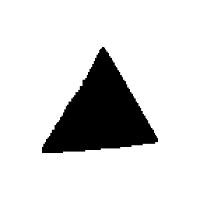
\includegraphics[width=\textwidth]{res/img/triangle.png}
    \end{subfigure}
    \begin{subfigure}[t]{0.2\textwidth}
        \centering
        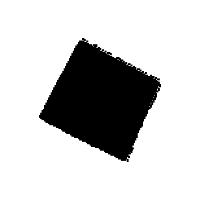
\includegraphics[width=\textwidth]{res/img/square.png}
    \end{subfigure}
    \\
    \begin{subfigure}[t]{0.2\textwidth}
        \centering
        
\includegraphics[width=\textwidth]{res/img/star.png}
    \end{subfigure}
    \begin{subfigure}[t]{0.2\textwidth}
        \centering
        
\includegraphics[width=\textwidth]{res/img/circle.png}
    \end{subfigure}
    \caption{Przykładowe kształty ze~zbioru treningowego używanego do~treningu i~oceny jakości klasyfikatorów}
    \label{fig:shapes}
\end{figure}

\subsection{Cel badań}

Kształty geometryczne wykazują pewien stopień regularności, co~powoduje, że do~ich rozpoznawania można próbować zastosować algorytmy dokładne.
Przykładem są zaimplementowane w~bibliotece OpenCV \cite{opencv}:
\begin{itemize}
    \item algorytm Suzukiego \cite{suzuki1985} do~wyznaczania konturów na~podstawie obrazów rastrowych,
    \item algorytm Douglasa-Peuckera \cite{douglas1973} do~upraszczania konturów i~redukcji liczby punktów.
\end{itemize}
Dzięki tym dwóm algorytmom można na~podstawie binarnego obrazu wejściowego wyznaczyć kontur kształtu --- łamaną zamkniętą przybliżającą kształt wyznaczony przez piksele kształtu na~tle.

Oprócz metod dokładnych, do~zagadnienia rozpoznawania można również użyć sieci neuronowych, które zamiast wiedzy dokładnej używają przygotowanych zbiorów treningowych oraz metod optymalizacji, aby~dokonać klasyfikacji.
Celem badań jest porównanie wydajności i~skuteczności wybranych metod.

\subsection{Wykorzystane techniki}

Do~zaimplementowania klasyfikatorów użyty został język skryptowy \textbf{Python} w~wersji 3.5.2.
Ponadto wykorzystane zostały dodatkowe biblioteki, wymienione w~tabeli~\ref{tbl:libraries}.
Podejście geometryczne opiera~się na~funkcjach udostępnianych przez \textbf{OpenCV}, podczas gdy sieci neuronowe stworzone zostały za~pośrednictwem API dostarczanego przez bibliotekę \textbf{Keras}.

\begin{table}[H]
    \begin{tabularx}{\textwidth}{|c|l|X|l|c|}
        \hline
        \textbf{Nr} & \textbf{Komponent, wersja} & \textbf{Opis} & \textbf{Licencja} & \\
        \hline
        \hline
        1 &
        Keras, 2.1.4 &
        Biblioteka udostępniająca API do~sieci neuronowych &
        MIT License &
        \cite{keras} \\
        \hline
        2 & 
        Matplotlib, 2.1.0 & 
        Umożliwia tworzenie wykresów &
        Matplotlib License &
        \cite{matplotlib} \\
        \hline
        3 & 
        NumPy, 1.13.3 &
        Używana do~efektywnych obliczeń na~wektorach $n$-wymiarowych &
        BSD License &
        \cite{numpy} \\
        \hline
        4 & 
        OpenCV, 3.3.0 &
        Biblioteka do~obróbki obrazów &
        New BSD License &
        \cite{opencv} \\
        \hline
        5 &
        pandas, 0.21.0 &
        Wspomaga ładowanie danych z~plików CSV oraz~ich analizę &
        BSD License &
        \cite{pandas} \\
        \hline
    \end{tabularx}
    \caption{Wykorzystane biblioteki wraz z~określeniem licencji}
    \label{tbl:libraries}
\end{table}

\subsubsection{Wycięcie kształtów z~tła}

Ponieważ projekt zakłada, że kolor kształtów jest zadany z~góry, do~ekstrakcji kształtów z~tła wystarczy zastosować operację progowania obrazu.
Pozwala ona na~zamianę obrazu w~kolorze na~obraz binarny.
Progowanie wykonywane jest w~przestrzeni kolorów HSV, która dobrze odwzorowuje podobieństwo odcieni barw; wystarczy zdefiniować przedział dla~parametru H, który określa sąsiedztwo tonalne żądanego koloru.

\subsubsection{Klasyfikator geometryczny}

Główną ideą działania klasyfikatora geometrycznego jest dopasowanie łamanej zamkniętej do~rozpoznanego kształtu i~analiza kształtu tej łamanej.

Do~odróżniania kształtów wykorzystywana jest przede wszystkim liczba wierzchołków w~wyznaczonym konturze.
Pozwala ona na~proste odróżnienie trójkątów, czworokątów i~dziesięciokątów od~pozostałych kształtów.
Ponadto, dla~każdego kształtu innego niż trójkąt, stosowane~są odpowiednie heurystyki:

\begin{itemize}
    \item W~przypadku kwadratów, sprawdzana jest proporcja wysokości do~szerokości kształtu (powinna być bliska jedności).
    Ponadto bok kwadratu wyznaczany jest na~podstawie pola i~obwodu figury; jeśli dwie wyznaczone wartości nie są bliskie sobie, kształt jest odrzucany.
    \item Rozpoznawanie gwiazd korzysta z~faktu, że wierzchołki parzyste i~nieparzyste gwiazdy znajdują~się w~innych odległościach od~środka figury.
    Zatem, jeśli odchylenie standardowe odległości od~środka wierzchołków parzystych i nieparzystych jest zbyt duże, figura jest odrzucana.
    \item Dla~kół, podobnie jak dla~kwadratów, promień koła wyznaczany jest dwukrotnie na~podstawie pola i~obwodu figury.
    W~przypadku zbyt dużej różnicy kształt nie jest klasyfikowany.
\end{itemize}

\subsubsection{Klasyfikatory oparte na~sieciach neuronowych}

Klasyfikatory oparte na~sieciach były trenowane na~podstawie zbioru treningowego \cite{shapes}.
Zostały opracowane dwa warianty sieci, operujące na~obrazie wejściowym rozmiarów $64 \times 64$:

\begin{itemize}
    \item W~pierwszym wariancie wejściowy binarny obraz dwuwymiarowy spłaszczany jest do~jednowymiarowego wektora, który przekazywany jest na~wejście sieci.
    Użyta sieć korzysta z~trzech warstw ukrytych z~funkcją aktywacji ReLU (ang. \emph{Rectified Linear Unit}).
    Ponadto, po~każdej warstwie ukrytej dodana jest warstwa \emph{dropout}, zapobiegająca zjawisku \emph{overfitting} \cite{srivastava2014}.

    Warstwa wyjściowa jako funkcji aktywacji używa funkcji \emph{softmax}.
    \item Drugi wariant korzysta z~pojedynczej warstwy konwolucyjnej z~rozmiarem okna $8 \times 8$ oraz warstwy \emph{dropout}.
    Wynik warstwy konwolucyjnej jest spłaszczany i~dostarczany do~warstwy wyjściowej z~funkcją \emph{softmax}.
\end{itemize}

\section{Instrukcja użytkowania aplikacji}

\subsection{Trenowanie sieci neuronowej}

\subsection{Przeprowadzenie kroswalidacji}

\subsection{Rozpoznawanie kształtów w~czasie rzeczywistym}

\section{Wyniki eksperymentalne}

\subsection{Kryteria oceny klasyfikatorów}

\subsection{Uzyskane wyniki}

\section{Podsumowanie}

\subsection{Możliwości dalszych badań}

\begin{thebibliography}{9}

    \bibitem{bishop1995}
        C.M. Bishop:
        \emph{Neural Networks for~Pattern Recognition}.
        Oxford University Press:
        Nowy Jork,
        1995.

    \bibitem{douglas1973}
        D.H. Douglas,
        T.K. Peucker,
        ,,Algorithms for the Reduction of~the~Number of~Points Required to~Represent a~Digitized Line or its Caricature'',
        \emph{Cartographica: The International Journal for Geographic Information and~Geovisualization},
        tom 10,
        s. 112--122,
        1973.

    \bibitem{keras}
        F. Chollet, Keras Team:
        Keras -- Deep Learning for humans. \\
        Oficjalna strona: \url{https://keras.io}
        [Dostęp 17~marca 2018]

    \bibitem{opencv}
        Intel Corporation, Willow Garage, Itseez:
        OpenCV -- Open Source Computer Vision. \\
        Oficjalna strona: \url{https://opencv.org}.
        [Dostęp 17~marca 2018]

    \bibitem{matplotlib}
        Matplotlib Development Team:
        Matplotlib. \\
        Oficjalna strona: \url{https://matplotlib.org}.
        [Dostęp 17~marca 2018]

    \bibitem{pandas}
        W. McKinney:
        pandas -- Python Data Analysis Library. \\
        Oficjalna strona: \url{https://pandas.pydata.org}.
        [Dostęp 17~marca 2018]

    \bibitem{shapes}
        S. Meschke:
        Four Shapes dataset. \\
        Dostępny: \url{https://www.kaggle.com/smeschke/four-shapes}.
        [Dostęp 17~marca 2018]

    \bibitem{srivastava2014}
        N. Srivastava,
        G. Hinton,
        A. Krizhevsky,
        I. Sutskever,
        R. Salakhutdinov,
        ,,Dropout: A Simple Way to Prevent Neural Networks from Overfitting'',
        \emph{Journal of Machine Learning Research},
        tom 15,
        s.~1929--1958,
        2014.

    \bibitem{suzuki1985}
        S. Suzuki,
        K. Abe,
        ,,Topological structural analysis of~digitized binary images''
        \emph{Computer Vision, Graphics and~Image Processing},
        tom 30,
        s.~32--66,
        1985.

    \bibitem{murty2015}
        M.N. Murty,
        V.S. Devi:
        \emph{Introduction to~Pattern Recognition and~Machine Learning}.
        World Scientific Publishing:
        Singapur,
        2015.

    \bibitem{numpy}
        T. Oliphant:
        NumPy. \\
        Oficjalna strona: \url{http://www.numpy.org}.
        [Dostęp 17~marca 2018]

\end{thebibliography}

\end{document}